\chapter{Мультиагентная система на основе Актор-Критик САУ} \label{chapt3}

Предложенный во второй главе метод построения САУ на основе обучения с подкреплением и метода Актор-Критик может быть использован для управления одним ОУ. Однако на практике нередко возникает запрос на управление одновременно несколькими ОУ, которые совместно должны выполнять некоторую задачу.

Мультиагентный подход к управлению несколькими ОУ предполагает отсутствие центрально органа управления или центрального агента. Децентрализация управления имеет ряд преимуществ, такие как автономность, устойчивость к отказам. Однако, для повышения качества управления такие системы должны обладать некоторым протоколом коммуникации. Агенты в такой системе могут обмениваться полученными знаниями, используя специальный язык. 

Предлагаемая в данной главе модификация метода Актор-Критик САУ призвана использовать обучение с подкреплением как основу для построения языка общения между агентами, действующими в одной среде и решающими одну задачу.

\section{Классификация} \label{subsect3_1}

Исследователи выделяют три вида мультиагентного обучения с подкреплением:
\begin{enumerate}
	\item полностью кооперативный,
	\item полностью конкурентный,
	\item смешанный.
\end{enumerate}




\begin{figure}[ht] 
	\center
	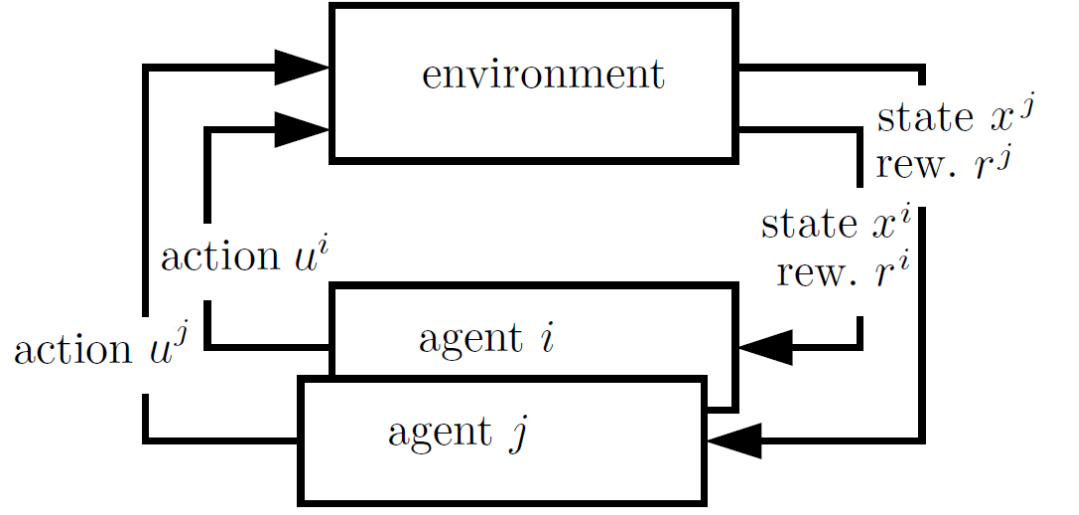
\includegraphics [scale=0.5] {multi/man}
	\caption{ Схема взаимодействия агентов и среды про обучении с подкреплением. } 
	\label{img:multi_main}  
\end{figure}

\section{Структура мультиагентной Актор-Критик САУ} \label{subsect3_2}

Как было сказано в начале третьей главы для построения мультиагентной системы необходимо создать канал для связи между агентами. Для решения данной задачи была разработана модифицированная версия Актор-Критик САУ. Основными модификациями являются:

\begin{enumerate}
	\item Блок Актор заменяется на 2 блока: Актор действия и Актор коммуникации. Актор действия выполняет функцию Актора выбирающей наиболее удачную стратегию воздействия на ОУ, а Актор коммуникации отвечает за выбор сообщения, передаваемого другим Агентам.
	\item ИНС Критика теперь представляет собой глубокую рекуррентную нейронную сеть.
	\item В вектор состояния, который принимает на вход агент добавлены сообщения других Агентов.
\end{enumerate}

\begin{figure}[ht] 
	\center
	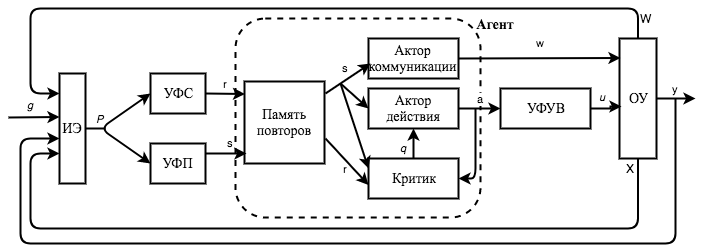
\includegraphics [scale=0.65] {ac_struct_multi}
	\caption{Структура мультиагнетной Актор-Критик САУ} 
	\label{img:ac_struct_multi}  
\end{figure}

(https://arxiv.org/pdf/1705.08926.pdf)
\subsection{Рекуррентные сети} \label{subsect3_2_1}
Сигнал с выходных нейронов или нейронов скрытого слоя частично передается обратно на входы нейронов входного слоя (обратная связь). Рекуррентная сеть Хопфилда «фильтрует» входные данные, возвращаясь к устойчивому состоянию и, таким образом, позволяет решать задачи компрессии данных и построения ассоциативной памяти. Частным случаем рекуррентных сетей являются двунаправленные сети. В таких сетях между слоями существуют связи как в направлении от входного слоя к выходному, так и в обратном. Классическим примером является Нейронная сеть Коско.

\subsection{Рекуррентный Критик} \label{sect3_2_2}

\section{Экспериментальные исследования} \label{sect3_4}


\subsection{Мультиагентное взаимодействие в задаче преследования} \label{subsect3_3_2}

Среда представляет собой поле 1000 на 1000 пикселей (рисунок 6), в которой действуют два мобильных робота. Цель роботов – перехватить две жертвы, причем так, чтобы каждый робот перехватил одну из жертв. Жертва считается захваченной, если робот приблизился к ее центру не дальше, чем 80 пикселей. На мобильных роботах установлено: 3 сонара, каждый из которых способен измерять расстояние до препятствия и его свойство – цвет, а также устрой-ство, показывающее относительный угол до каждой из жертв. Кинематические свойства робо-тов описываются системой уравнения для машины Дубинса []. Робот также способен «слышать» то, что ему говорит партнер. Управление роботом осу-ществляется с помощью выбора одной из трех команд: «налево», «прямо», «направо». Помимо управления движением возможно использование информационного канала между агентами, которое реализовано в виде обмена словами, которых в данной среде доступно 3. Выбор раз-мера пространства слов равным 3 обусловлено предположением, что вполне достаточно для выполнения данной задачи 3 вида сообщений {«Я выбрал или настиг цель 1», «Я выбрал или настиг цель 2», «Я еще не определился с целью»}

\begin{figure}[ht] 
	\center
	\includegraphics [scale=1] {dubins_multi/image1}
	\caption{Визуализация среды, объекты: маленькие кружки - роботы, черные точки - линии действия сонаров, большие кружки – цели.} 
	\label{img:dubins_multi}  
\end{figure}

\begin{table} [htbp]
	\centering
	\caption{ Архитектуры ИНС Актора и Критика }
	\label{Ts0Sib4}%
	\begin{tabular}{|p{0.1in}|p{2in}|p{2in}|p{2in}|} \hline 
		\textit{} & \multicolumn{2}{|p{2.3in}|}{\textit{Структура Актора}} & \textit{Структура Критика} \\ \hline 
		& \textit{Актор действия} & \textit{Актор коммуникации} &  \\ \hline 
		1 & Полносвязный: 256 & Полносвязный: 1024 & LSTM 16/4 \\ \hline 
		2 & Дропаут: 20\% & Дропаут: 10\% & LSTM 16 \\ \hline 
		3 & РЕЛУ [4] & РЕЛУ & Полносвязный: 1 \\ \hline 
		4 & Полносвязный: 256 & Полносвязный: 1024 &  \\ \hline 
		5 & Дропаут: 20\% & Дропаут: 10\% &  \\ \hline 
		6 & РЕЛУ & РЕЛУ &  \\ \hline 
		7 & Полносвязный: 3 & Полносвязный: 3  &  \\ \hline 
	\end{tabular}
\end{table}

\begin{figure}[ht] 
	\center
	\includegraphics [scale=1] {dubins_multi/image2}
	\caption{Схема взаимодействия агентов.} 
	\label{img:dubins_multi2}  
\end{figure}

Расчет награды r происходит по следующим правилам:
\begin{enumerate}
	\item Если угол между роботом и целью меньше 15$ {^\circ} $ и эту цель не захватил другой робот, то r= 0.8
	\item Если робот захватил цель, то r = 0.8
	\item Если оба робота захватили обе цели, то r = 1 – победа
	\item Если робот врезается в партнера или в границу среды, то r = -1 – поражение
	\item Во всех остальных случаях r = -0.1
\end{enumerate}

Результаты:

Сравнение обученного агента производилось с жадным алгоритмом в нескольких режи-мах функционирования среды: со статической жертвой, со случайно двигающейся жертвой, а также с разным минимальным радиусом разворота робота – машины Дубинса. Качество оценивалось долей успешный запусков относительно общего количества, для каждого эксперимента было произведено по 500 запусков. 
Как видно из таблицы 2 качество работы обученного агента сопоставимо с качеством жадного алгоритма. Результаты в таблице 3 показывают, что коммуницирующие роботы решают задачу лучше, чем некоммуницирующие, из чего можно сделать вывод, что данный подход к обучению коммуникации между роботами имеет место быть. Так же в [9,10] представлены результаты похожих работ, что показывает перспективность подобного подхода.

\begin{table} [htbp]
	\centering
	\caption{ Доли успешных запусков для жадного алгоритма и модели Актор-Критик }
	\label{Ts0Sib5}%
	\begin{tabular}{|p{2.7in}|p{1.5in}|p{1.5in}|} \hline 
		& \textbf{Жадный алгоритм} & \textbf{Актор-Критик САУ} \\ \hline 
		\textit{Статическая/радиус 50} & \textit{0,61} & \textit{0,59} \\ \hline 
		\textit{Статическая/радиус 100} & \textit{0,55} & \textit{0,58} \\ \hline 
		\textit{Динамическая/радиус 50} & \textit{0,60} & \textit{0,60} \\ \hline 
		\textit{Динамическая/радиус 100} & \textit{0,60} & \textit{0,60} \\ \hline 
	\end{tabular}
\end{table}

\begin{table} [htbp]
	\centering
	\caption{ Сравнение коммуницирующих и некоммуницирующих роботов }
	\label{Ts0Sib6}%

	\begin{tabular}{|p{4.0in}|p{0.8in}|} \hline 
		\textit{Всегда передается одно и тоже слово} & \textit{0,41} \\ \hline 
		\textit{Передается случайное слово} & \textit{0,51} \\ \hline 
		\textit{Актор коммуникации} & \textit{0,59} \\ \hline 
	\end{tabular}
\end{table}

\section{Метод общения между роботами в реальном мире} \label{sect3_5}

Задача коммуникации роя роботов не является нерешённой (работы об архитектуре mesh сетей [2, 3]). Так, существуют различные подходы, например, в [4] предлагается построение системы, базирующейся на инфракрасных трансмиттерах, но такая система работает в пределах видимо-сти. Существуют радиопротоколы, поддерживающие построение сетей с ячеистой топологией, например, ZigBee [5] (вариант системы, построенной на ZigBee [6]), но стоимость такого чипа высока и составляет порядка $25, в то время как стоимость используемого в работе Wi-Fi чипа ESP8266 не превышает $3. Также протокол Wi-Fi гораздо более распространён чем ZigBee, что является несомненным преимуществом, а также позволяет не использовать дополнительное оборудование для приёма информации от роботов на хосте. Наконец, немаловажным аспектом в пользу выбора чипа ESP8266 стал тот факт, что он содержит на борту дискретные порты ввода-вывода, аналого-цифровой преобразователь, драйверы протоколов SPI, UART, а это в дальнейшем может стать основанием к разработке ро-бота, который управляется только этим чипом без дополнительных микроконтроллеров [7]. Недостатком этого чипа, по отношению к ZigBee, яв-ляется достаточно большое энергопотребление. 
В данной работе ставилась задача построения сети с ячеистой топологией, на основе технологии Wi-Fi, способной возвращать оценочные значения расстояний между узлами базируясь на информации об уровне принимаемого сигнала. Тестирование выполнялось на совокупности из 4х роботов (рис. 1), которые обменивались информацией о своём состоянии и оценкой расстояний до соседей. Целью данной работы в том числе являет-ся построение такой системы, которая была бы применима для разных ти-пов автономных роботов: летающих, ездящих – обладающих UART интерфейсом.

\begin{figure}[ht] 
	\center
	\includegraphics [scale=1] {comm/image1}
	\caption{Четыре трёхколёсных робота, каждый с приводом на 2 колеса.} 
	\label{img:dubins_multi2}  
\end{figure}

Функционирование сети базируется на работе протокола TCP, кото-рый гарантирует доставку сообщения до принимающей стороны. Модуль ESP8266 обладает способностью находиться в двух состояниях одновре-менно: как точка доступа и как клиент, поэтому нет необходимости пере-ключаться между этими двумя состояниями. Также особенностью данного алгоритма является то, что сообщения рассылаются широковещательно и сам узел решает, что ему делать с полученной информацией. За основу был взят код библиотеки ESP8266WiFiMesh, написанный Julian Fellх[8]. 

\begin{figure}[ht] 
	\center
	\includegraphics [scale=1] {comm/image2}
	\caption{Блок-схема работы алгоритма.} 
	\label{img:dubins_multi2}  
\end{figure}

Блок-схема на рисунке 2 показывает общую схему функционирова-ния алгоритма ячеистой сети:
1.	Блок 1 алгоритма отвечает за инициализацию узла, присвоение ему имени в соответствии с шаблоном: «Robot»+N (где N – это уникаль-ный номер узла). Префикс «Robot» необходим при поиске сетей, и только точки доступа с таким префиксом являются участниками сети. Также на этом этапе создаётся Wi-Fi точка доступа с аналогичным именем и фиксированным IP адресом (192.168.4.1) и запускается TCP сокет на порту 4011.
2.	Блок 2 отвечает за приём информации от робота и формирование пакета. Информация, содержащая RSSI подключения, будет добавлена в блоках 3 и 4.
3.	Блок 3 отвечает за обработку подключений к данному узлу. Если в течение определённого времени произошло подключение стороннего узла к сокету и был получен пакет информации, то в ответ отсылается заранее подготовленная информация от данного юнита. Если такого подключения нет, то происходит переход к следующему блоку.
4.	Блок 4 начинает сканирование Wi-Fi сетей и отбрасывает все сети, которые не начинаются с префикса «Robot». Ко всем оставшимся сетям текущий узел пытается подключиться и обменяться сообщениями. Все повторяется, начиная с блока 2.

Конечно, в данном алгоритме присутствует некая избыточность: широковещательные передачи, обмен сообщениями, но это нисколько не мешает ему адекватно работать.

Структура передаваемых данных
Передаваемая информация включает в себя телеметрические данные о работе систем автономного робота, информацию о силе принимаемого сигнала между двумя подключенными друг к другу узлами

\begin{table} [htbp]
	\centering
	\caption{ Таблица. Структура данных }
	\label{Ts0Sib5}%
	\begin{tabular}{|p{3.3in}|p{1.0in}|} \hline 
		Описание & Тип \\ \hline 
		Уникальный идентификатор узла & integer \\ \hline 
		Структура данных, содержащая информацию о значении RSSI, а также идентификаторы узлов, между которыми велась передача & Особый \\ \hline 
		Уровень заряда батареи в процентах & float \\ \hline 
		Прогнозируемое время работы в минутах & integer \\ \hline 
		Данные GPS о геолокации & string \\ \hline 
		Время, полученное от GPS спутников & string \\ \hline 
		Время от часов реального времени, установленных на роботе & string \\ \hline 
		Значение таймера в мс, запущенного с начала работы узла & long integer \\ \hline 
		Температура окружающего воздуха в С$\circ$ & float \\ \hline 
		Скорость движения в м/с & float \\ \hline 
		Структура данных, содержащая углы Эйлера (крен, тангаж, рысканьне) в градусах & Особый \\ \hline 
		Показания Барометра в мм рт. столба & float \\ \hline 
	\end{tabular}
\end{table}

Структура данных, представленная в таблице 1 выше, содержит информацию, которую можно использовать для мониторинга работы роя роботов, а также для построения карты их относительного положения. Данная структура несколько избыточна для роботов, участвовавших в этой работе, но она разрабатывалась на будущее.
В данной работе был предложен вариант построения сети с ячеистой топологией на основе Wi-Fi с использованием модуля ESP8266 с возможностью оценивания взаимного расположения узлов на основе информации о силе принимаемого сигнала. В ходе работе была протестирована сеть, состоящая из четырёх узлов, и результат тестирования можно считать успешным. Тестирование производилось на базе четырёх мобильных ро-ботов (рис. 1), которые обменивались информацией о своём состоянии.
Такого рода системы могут найти своё применение в при коммуникации разного типа роботов, наземных или воздушных, в условиях, когда не всегда удаётся обеспечить связь каждого робота с центральным узлом.

\section{Склад} \label{sklad}

\section{Запуск агента на мобильном устройстве} \label{agent_mobile}

Применение нейросетевых агентов в на мобильных устройствах всегда сопряжено с задачей удовлетворения требований по скорости работы, так как в основе работы глубоких нейронных сетей лежат операции с большими матрицами. 

В качестве платформы для управления мобильным агентом были выбраны устройства Apple Iphone 6s. Данное устройство имеет современный процессор A9 со встроенным графическим сопроцессором.

\begin{figure}[ht] 
	\center
	\includegraphics [scale=0.25] {a9}
	\caption{Структура процессора А9.} 
	\label{img:a9}  
\end{figure}

\begin{figure}[ht] 
	\center
	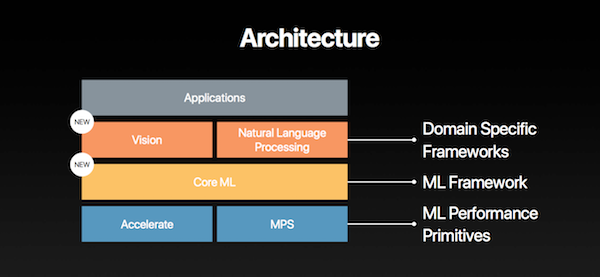
\includegraphics [scale=0.7] {coreml}
	\caption{Архитектура программного решения для ускорения нейросетей от Apple.} 
	\label{img:coreml}  
\end{figure}

Нейросетевой агент Актор-Критик использует для фреймворк Keras, который поддерживается Coremltools - особый инструмент для транслирования весов нейронной сети в формат, с которым может работать Coreml\cite{vakbib1, vakbib2}.

\begin{figure}[ht] 
	\center
	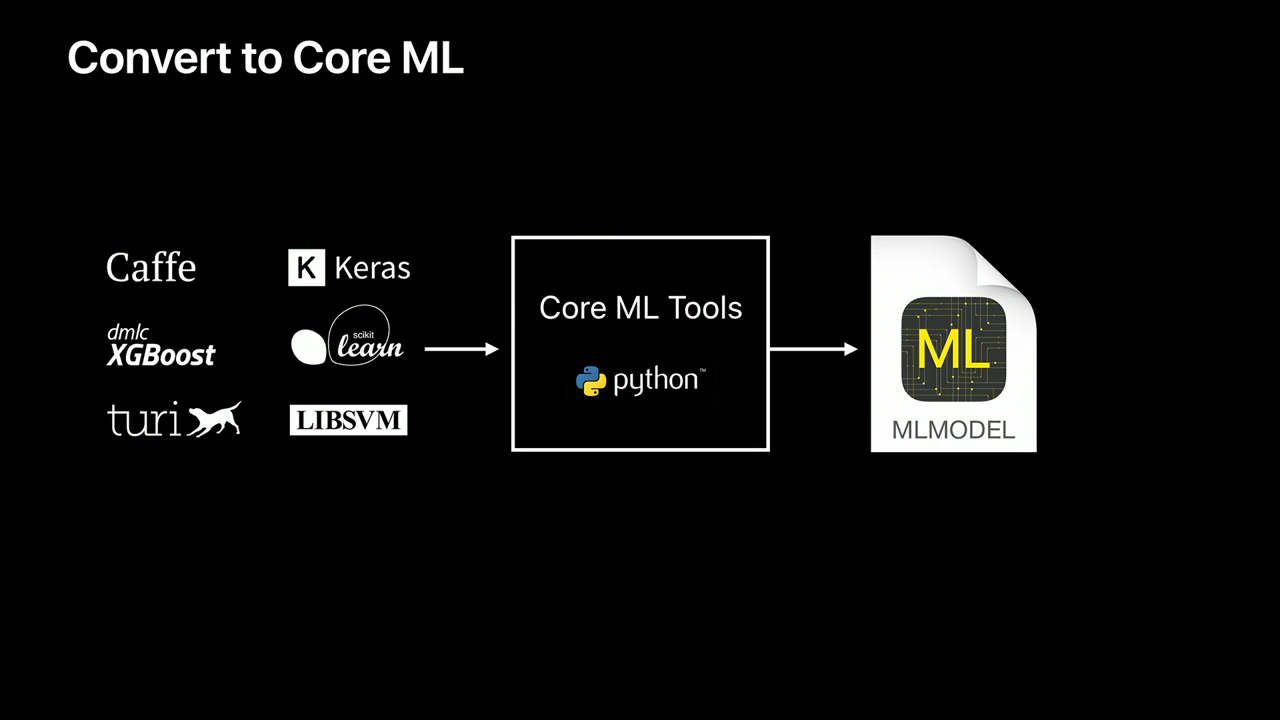
\includegraphics [scale=0.4] {coremltools}
	\caption{Архитектура программного решения для ускорения нейросетей от Apple.} 
	\label{img:coremltools}  
\end{figure}

\begin{table} [htbp]
	\centering
	\caption{ Тайминги работы агента на различных устройствах }
	\label{table_coremls}%
	\begin{tabular}{|p{2.0in}|p{1.5in}|} \hline 
		& \textbf{Время работы} \\ \hline 
		\textit{CPU Intel 2600k} & \textit{0}  \\ \hline 
		\textit{GPU Titan X Maxwell} & \textit{0}  \\ \hline 
		\textit{Iphone 6s} & \textit{0}  \\ \hline 
		\textit{Iphone 7} & \textit{0}  \\ \hline 
	\end{tabular}
\end{table}





\section{Основные выводы по главе 3} \label{vivod3}
 
\begin{enumerate}
	\item Приведено описание схемы Актор-Критик САУ, использующей в своей основе глубокие нейронные сети для аппроксимаций функций Актора и Критика.
	\item Приведено описание алгоритмов работы каждого блока схемы Актор-Критик САУ
	\item Приведено описание разработанного программного средства для моделирования работы Актор-Критик САУ в различных конфигурациях с разными средами.
	\item Приведены результаты экспериментальных исследований, в процессе которых изучалось применение Актор-Критик САУ для различных объектов управления.
\end{enumerate}

\clearpage
\clearpage
